\textbf{Ejemplo 2}\\

Supongamos que para un inversionista la TIO es del 3\% periodo anual vencido, con esta tasa seleccionar uno de los siguientes proyectos:\\

\textbf{Proyecto A}\\
Requiere de una inversión inicial de  COP  1.160.000, producirá un ingreso de  COP  1.000.000 en el primer año y en cada uno de los años 2 al 6 producirá ingresos de  COP  50.000.\\

\textbf{Proyecto B}\\
Requiere de una inversión inicial de  COP  1.160.000 y al final del año 6 producirá un ingreso de  COP  1.500.000.
\\

\textbf{Solución.}\\
%La tabla ira centrada
\begin{center}
	\renewcommand{\arraystretch}{1.5}% Margenes de las celdas
	%Creación de la cuadricula de 3 columnas
\begin{longtable}[H]{|c|c|c|}
		%Creamos una linea horizontal
\hline
		%Definimos el color de la primera fila
\rowcolor[HTML]{FFB183}
%%%%% INICIO ASIGNACIÓN PERÍODO FOCAL %%%%%%%
  %%%%%%%%%% INICIO TITULO
  %Lo que se hace aquí es mezclar las 3 columnas en una sola
  \multicolumn{3}{|c|}{\cellcolor[HTML]{FFB183}\textbf{1. Asignación período focal}}   \\ \hline
  %%%%%%%%%% FIN TITULO
  %%%%% INICIO DECLARACIÓN DE VARIABLES %%%%%%%
  \multicolumn{3}{|c|}{$pf = 0 pav$}   \\ \hline
  
%%%%%%%%%%% INICIO TITULO
\rowcolor[HTML]{FFB183}
\multicolumn{3}{|c|}{\cellcolor[HTML]{FFB183}\textbf{2. Declaración de variables}}    \\ \hline
%%%%%%%%%%% FIN TITULO
%%%%%%%%%%% INICIO MATEMÁTICAS

$\textbf{Proyecto A}$                                     & \multicolumn{2}{c|}{$ \textbf{Proyecto B} $} \\
$n = 6 pav \hspace{0.3cm} $	& \multicolumn{2}{c|}{$ n = 6 pav $} \\
$\text{Inversión inicial} =  COP  1.160.000 $	&	\multicolumn{2}{c|}{ $\text{Inversión inicial} =  COP  1.160.000 $ } \\
$\text{Ingreso al año 1} =  COP  1.000.000 $	&	\multicolumn{2}{c|}{ $ \text{Ingreso final del año } =  COP  1.500.000 $ } \\ 
$ \text{Ingreso al año 2 al 6} =  COP  50.000 $	&	\multicolumn{2}{c|}{ $ i = 3\% pav = TIO $ }
\\
$ i = 3\% pav = TIO $	&	\multicolumn{2}{c|}{ $ $ }
\\
\hline
%%%%%%%%%% FIN MATEMÁTICAS
		%%%%% INICIO FLUJO DE CAJA
\rowcolor[HTML]{FFB183}
\multicolumn{3}{|c|}{\cellcolor[HTML]{FFB183}\textbf{3. Diagrama de flujo de caja}} \\ \hline
		%Mezclamos 3 columnas y pondremos el dibujo
		%%%%%%%%%%%%% INSERCIÓN DE LA IMAGEN
		%Deberán descargar las imágenes respectivas del drive y pegarlas en la carpeta
		%n_capitulo/img/ejemplos/1/capitulo1ejemplo1.pdf  (el /1/ es el numero del ejemplo)
\multicolumn{3}{|c|}{ 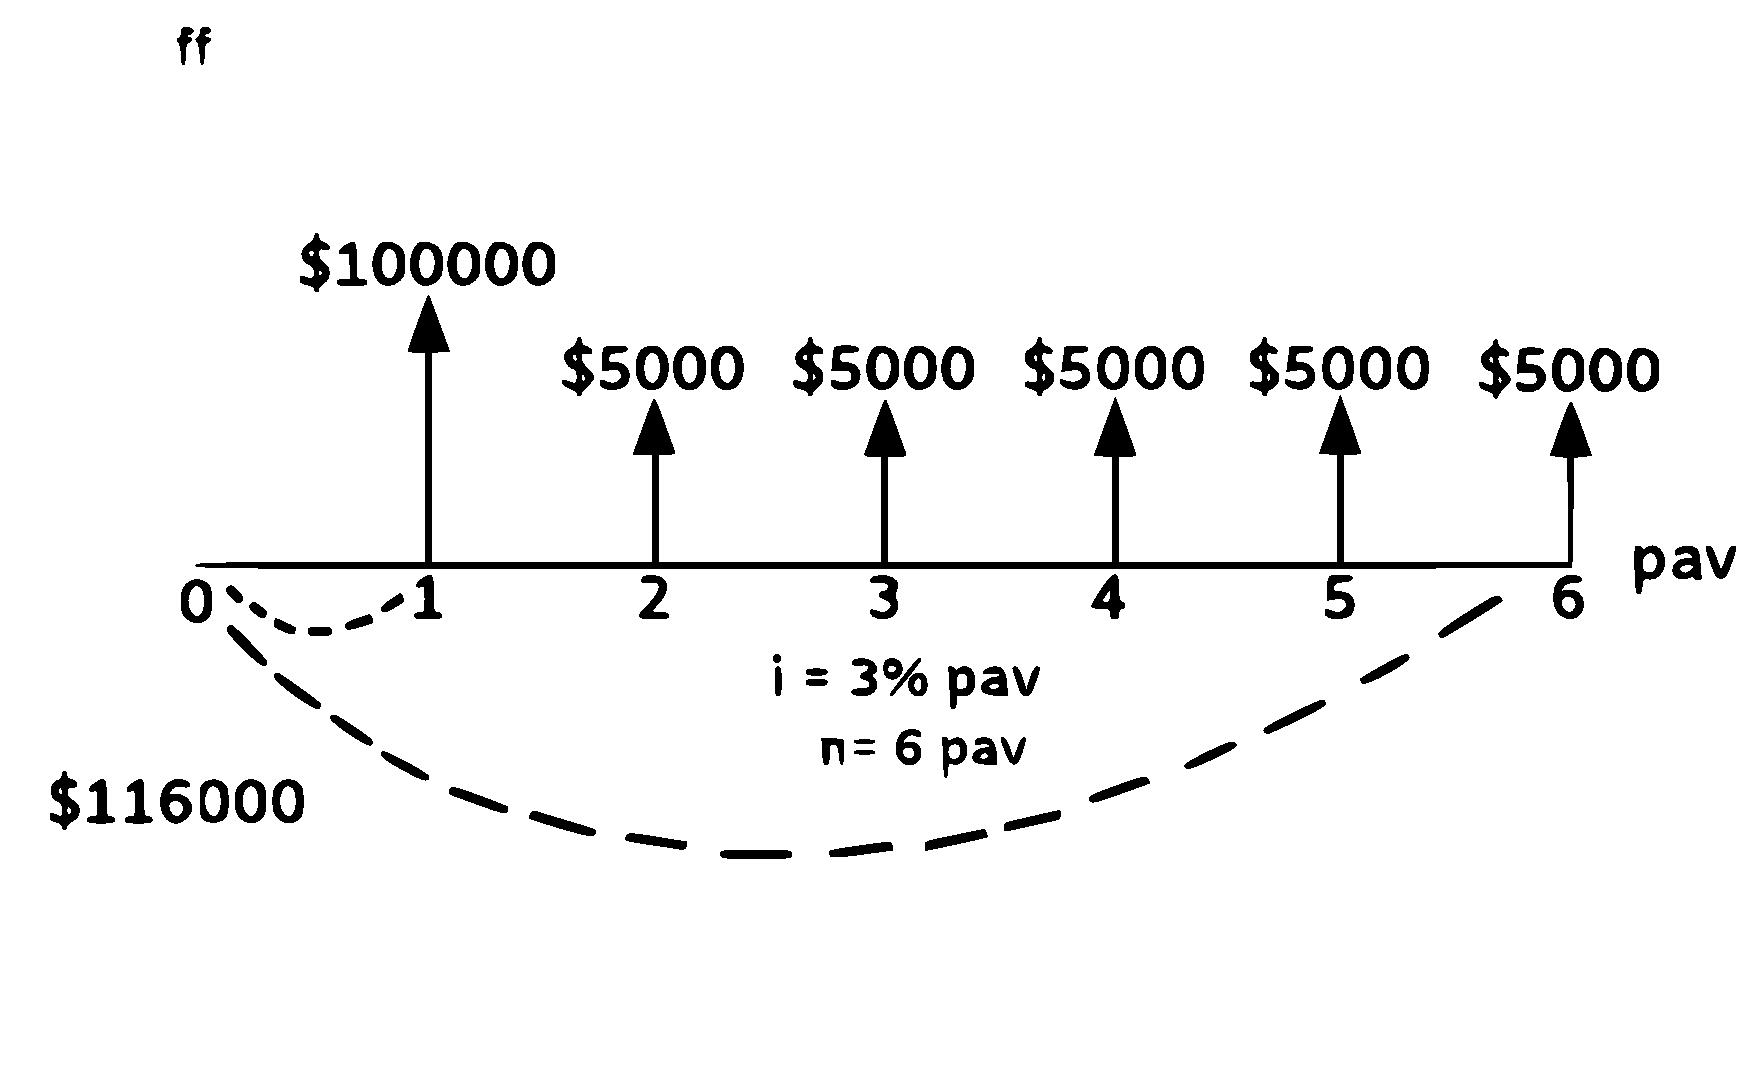
\includegraphics[scale=0.4, trim=-5 -5 -5 -5]{Graf4Cap11.pdf} }   
   \\ 
\multicolumn{3}{|c|}{ 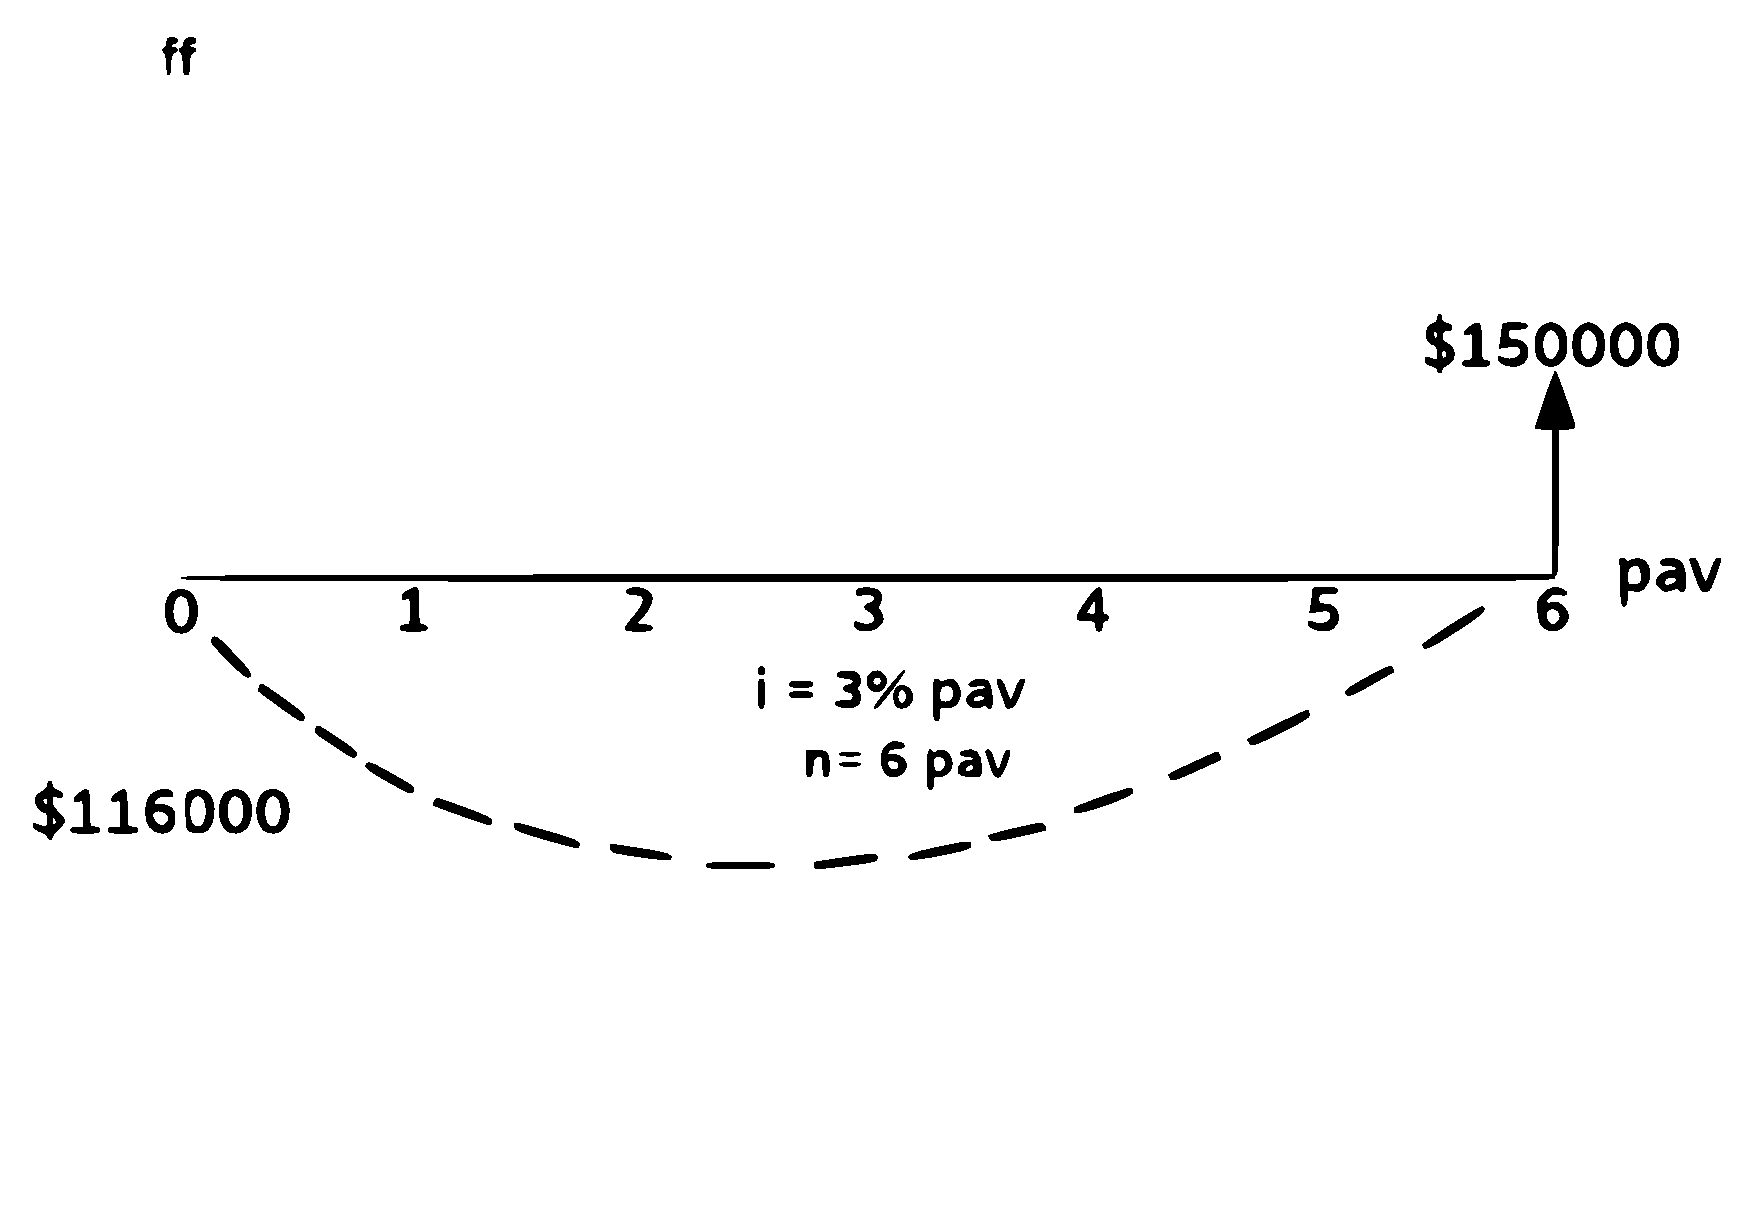
\includegraphics[scale=0.4, trim=-5 -5 -5 -5]{Graf5Cap11.pdf} }  
   \\\hline
		%%%%%%%%%%%%% FIN INSERCIÓN DE IMAGEN
		%%%%%FIN FLUJO DE CAJA
		
		
		
		%%%%% INICIO DECLARACIÓN FORMULAS
		%%%%%%%%%%% INICIO TITULO
\rowcolor[HTML]{FFB183}
\multicolumn{3}{|c|}{\cellcolor[HTML]{FFB183}\textbf{4. Declaración de fórmulas}}    \\ \hline
		%%%%%%%%%%% FIN TITULO
		%%%%%%%%%%% INICIO MATEMÁTICAS
\multicolumn{3}{|c|} {VPN =	$\sum F_{n}(1+i)^{-n}$   Valor presente neto.}   \\ \hline	
	
		%%%%%%%%%% FIN MATEMÁTICAS
		%%%%%% INICIO DESARROLLO MATEMÁTICO
\rowcolor[HTML]{FFB183}
		%%%%%%%%%%INICIO TITULO
\multicolumn{3}{|c|}{\cellcolor[HTML]{FFB183}\textbf{5. Desarrollo matemático}}       \\ \hline
		%%%%%%%%%% FIN TITULO
		%%%%%%%%%% INICIO MATEMÁTICAS
		\multicolumn{3}{|c|}{$ VPN(A) = -  COP  1.160.000 +  COP  1.000.000(1+0.03)^{-1} +  COP  50.000(\frac{1-(1+0.03)^{-5}}{0.03})(1+0.03)^{-1} =  COP  33.189,67 $} \\
		\multicolumn{3}{|c|}{$ VPN(B) = -  COP  1.160.000 +  COP  1.500.000(1+0.03)^{-6} =  COP  96.226,29 $}   \\
	    \hline
				
		%%%%%%%%%% FIN MATEMÁTICAS
		%%%%%% FIN DESARROLLO MATEMÁTICO
		%%%%%% INICIO RESPUESTA
\rowcolor[HTML]{FFB183}
		%%%%%%%%%%INICIO TITULO
\multicolumn{3}{|c|}{\cellcolor[HTML]{FFB183}\textbf{6. Respuesta}}   \\ \hline
		%%%%%%%%%% FIN TITULO
		%%%%%%%%%% INICIO RESPUESTA MATEMÁTICA
		
\multicolumn{3}{|c|}{ \text{El análisis usando el VPN indica que es mejor el proyecto B puesto que VPN(B)>VPN(A)} } \\ 
\hline
		
		
		%%%%%%%%%% FIN MATEMÁTICAS
		%%%%%% FIN RESPUESTA
	\end{longtable}
	%Se crean dos lineas en blanco para que no quede el siguiente texto tan pegado
	%\newline \newline %USARLO SI CREES QUE ES NECESARIO
\end{center}
%%%%%%%%%%%%%%%%%%%%%%%%%%FIN EJERCICIO 1 %%%%%%%%%%%%%%%%%%%%%%%%%%%
